% Compile with latex, then dvisvgm --no-fonts --exact --bbox=min.
\documentclass[tikz,border=5pt]{standalone}
\begin{document}
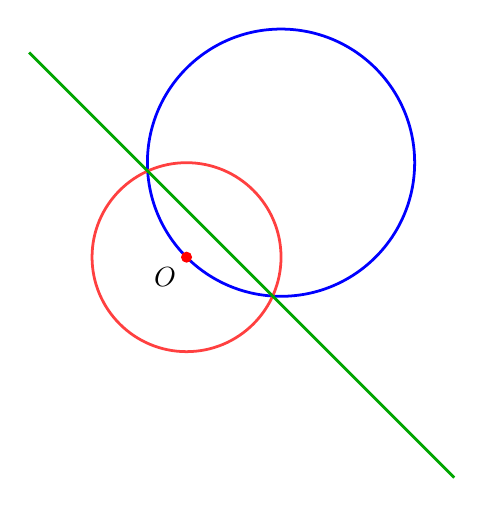
\begin{tikzpicture}[line width=1pt]
  % The blue circle has centre (1.2,1.2) and passes through O.
  % Inversion in radius 1.2 maps it to 1.2x+1.2y=1.2^2/2.
  \draw[blue] (1.2,1.2) circle ({sqrt(2)*1.2});
  \draw[red!75] (0,0) circle (1.2);
  \draw[green!65!black] (-2,2.6) -- (3.4,-2.8);
  \fill[red] (0,0) circle (2pt) node[below left,black] {$O$};
\end{tikzpicture}
\end{document}
